\documentclass[12pt,a4paper]{article}
\usepackage[utf8]{inputenc}
\usepackage[spanish]{babel}
\usepackage{amsmath}
\usepackage{amsfonts}
\usepackage{amssymb}
\usepackage{graphicx}
\usepackage[left=2cm,right=2cm,top=2cm,bottom=2cm]{geometry}

\usepackage{enumitem}
\usepackage{algorithm}
\usepackage{algorithmic}
\usepackage[hidelinks]{hyperref}

\usepackage{tikz}

\usepackage{subcaption}
\usepackage{pgfplots}

% Para la tabla
\usepackage[normalem]{ulem}
\useunder{\uline}{\ul}{}


\author{Ignacio Aguilera Martos}
\title{Práctica 2 \\ Técnicas de los Sistemas Inteligentes}
\date{\today}

\setlength{\parindent}{0cm}
\setlength{\parskip}{10px}


\begin{document}
	\maketitle

	\tableofcontents

	\newpage

\section{Ejercicio 1}

El primero de los apartados nos pide definir los objetos, personajes y demás tipos utilizados en el dominio. Los tipos que yo he representado son zona, orientación, agente, princesa, principe, bruja, profesor, leonardo, oscar, manzana, rosa, algoritmo, oro, personaje, objeto y posicionable.

El diagrama de tipos que he empleado es un árbol de la forma:

\begin{figure}[H]
	\centering
	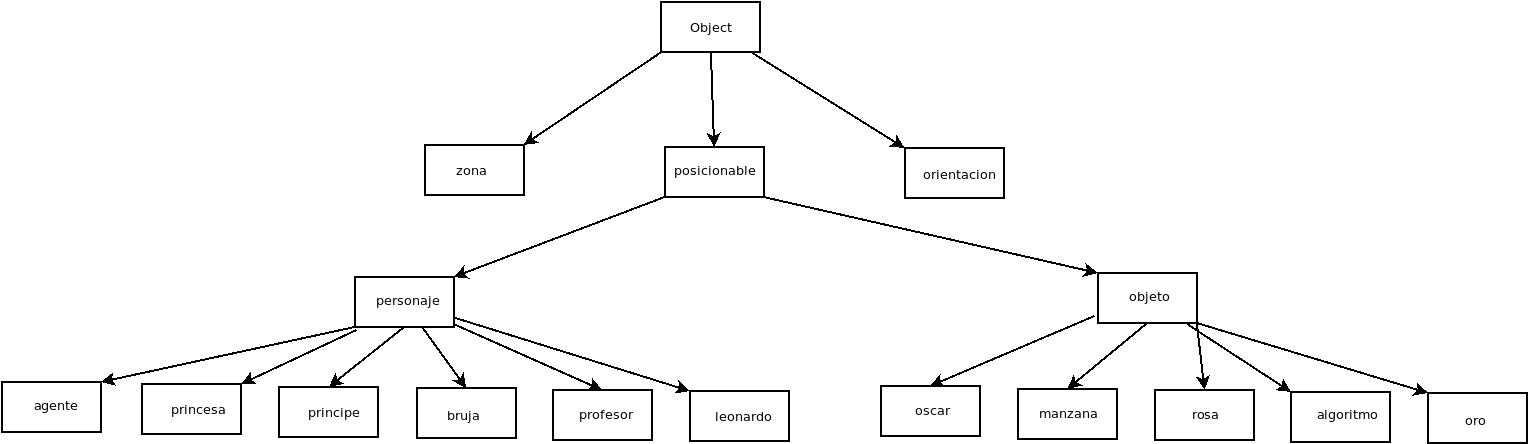
\includegraphics[scale=0.32]{./Imagenes/diag-ej1.png}
	\caption{Diagrama de tipos}
\end{figure}

En cuanto a los predicados que he tomado para resolver el ejercicio son:

\begin{itemize}
	\item (en ?x - posicionable ?y - zona): este predicado lo que nos indica es que el objeto o personaje ?x está en la zona ?y.
	\item (orientado ?a - personaje ?ori - orientacion): este predicado nos dice que el personaje (incluido el propio agente) ?a está orientado según la orientación ?ori.
	\item (conectado ?z1 ?z2 - zona ?ori - orientacion): este predicado nos dice que las zonas ?z1 y ?z2 están conectadas por la orientación ?ori, esto es si z2 está a la derecha de z1 entonces están conectadas por el este, si z2 está debajo de z1 entonces z1 está conectada a z2 por el sur y así para el resto de orientaciones.
	\item (manovacia ?a - agente): este predicado nos dice si el agente ?a tiene o no la mano vacía para llevar un objeto.
	\item (enlamano ?a - agente ?obj - objeto): este predicado nos dice que el agente ?a tiene un objeto ?obj en la mano.
	\item (tieneobjeto ?per - personaje): este predicado nos indica que el personaje ?per tiene un objeto.
\end{itemize}

Cabe decir que además de los predicados y tipos he definido 4 constantes para las orientaciones que son este, oeste, norte y sur.

Para las acciones las he definido de la siguiente forma:

\begin{itemize}
	\item girar-izquierda: es la acción que nos permite rotar hacia la izquierda, requiere como único parámetro un agente y el efecto es, comprobando la orientación actual del agente cambiar dicha orientación de forma adecuada al giro a la izquierda.
	\item girar-derecha: es la misma acción que girar a la izquierda pero cambiando el sentido de la rotación.
	\item ir: recibe como parámetros un agente, dos zonas y una orientación. Como precondiciones establecemos que el agente esté en la primera de las posiciones, que el agente esté orientado según la orientación dada y que las zonas estén conectadas en esa dirección. El efecto de esta acción es que el agente pasa a estar en la segunda zona y deja de estar en la primera.
	\item coger: esta acción recibe como parámetros un agente, una zona y un objeto. Se pide como precondición que el agente esté en la zona, el objeto también y que el agente tenga la mano vacía. Como efecto se produce que el agente deja de tener la mano vacía, el objeto deja de estar en la zona y pasa a estar en la mano del agente.
	\item dejar: recibe como parámetros un agente, una zona y un objeto. Como precondiciones se pide que el agente esté en la posición y tenga el objeto en la mano. El efecto que se produce es que el objeto pasa a estar en la zona y desaparece de la mano del agente y éste pasa a tener la mano vacía.
	\item entregar: recibe como parámetros un agente, una zona, un objeto y un personaje. Como precondiciones se pide que el agente esté en la zona, el personaje también y que el agente tenga el objeto en la mano. El efecto producido es que el agente deja de tener el objeto en la mano, pasa a tener la mano vacía y el objeto pasa a tenerlo el personaje.
\end{itemize}

Lo siguiente que se nos pide es que planteemos de forma manual un problema con 25 zonas, 5 personajes mas el agente y 5 objetos. El objetivo será que cada uno de los 5 personajes tenga un objeto.

La disposición del mapa que he dado es la siguiente:

\begin{table}[H]
	\begin{tabular}{|l|l|l|l|l|l|l|l|}
		\hline
		z1{[}agente{]} & z2  & z3{[}princesa{]}  & z4               & z5{[}principe{]}  &               &     &                    \\ \hline
		z6{[}oro{]}    & z7  & z8{[}oscar{]}     & z9               & z10{[}leonardo{]} &               &     &                    \\ \hline
		z11{[}bruja{]} & z12 & z13               & z14{[}manzana{]} & z15               &               &     & z25                \\ \hline
		z16            & z17 & z18{[}profesor{]} & z19              & z20               & z21{[}rosa{]} & z22 & z23{[}algoritmo{]} \\ \hline
		&     &                   &                  &                   &               &     & z24                \\ \hline
	\end{tabular}
\end{table}

Partimos además de que el agente está orientado hacia el norte, tiene la mano vacía y el objetivo es que todos los personajes tengan un objeto.

El problema es resoluble y ff nos da la solución:
\begin{enumerate}
	\item GIRAR-DERECHA AGENTE1
	\item IR AGENTE1 Z1 Z2 ESTE
	\item IR AGENTE1 Z2 Z3 ESTE
	\item GIRAR-DERECHA AGENTE1
	\item IR AGENTE1 Z3 Z8 SUR
	\item COGER AGENTE1 Z8 OSCAR1
	\item IR AGENTE1 Z8 Z13 SUR
	\item IR AGENTE1 Z13 Z18 SUR
	\item GIRAR-DERECHA AGENTE1
	\item GIRAR-DERECHA AGENTE1
	\item ENTREGAR AGENTE1 Z18 OSCAR1 PROFESOR1
	\item IR AGENTE1 Z18 Z13 NORTE
	\item GIRAR-IZQUIERDA AGENTE1
	\item IR AGENTE1 Z13 Z12 OESTE
	\item IR AGENTE1 Z12 Z11 OESTE
	\item GIRAR-DERECHA AGENTE1
	\item IR AGENTE1 Z11 Z6 NORTE
	\item GIRAR-DERECHA AGENTE1
	\item GIRAR-DERECHA AGENTE1
	\item COGER AGENTE1 Z6 ORO1
	\item IR AGENTE1 Z6 Z11 SUR
	\item GIRAR-DERECHA AGENTE1
	\item GIRAR-DERECHA AGENTE1
	\item GIRAR-DERECHA AGENTE1
	\item ENTREGAR AGENTE1 Z11 ORO1 BRUJA1
	\item IR AGENTE1 Z11 Z12 ESTE
	\item IR AGENTE1 Z12 Z13 ESTE
	\item GIRAR-IZQUIERDA AGENTE1
	\item IR AGENTE1 Z13 Z8 NORTE
	\item IR AGENTE1 Z8 Z3 NORTE
	\item GIRAR-DERECHA AGENTE1
	\item IR AGENTE1 Z3 Z4 ESTE
	\item GIRAR-DERECHA AGENTE1
	\item IR AGENTE1 Z4 Z9 SUR
	\item IR AGENTE1 Z9 Z14 SUR
	\item GIRAR-IZQUIERDA AGENTE1
	\item GIRAR-IZQUIERDA AGENTE1
	\item COGER AGENTE1 Z14 MANZANA1
	\item IR AGENTE1 Z14 Z9 NORTE
	\item IR AGENTE1 Z9 Z4 NORTE
	\item GIRAR-DERECHA AGENTE1
	\item IR AGENTE1 Z4 Z5 ESTE
	\item GIRAR-DERECHA AGENTE1
	\item IR AGENTE1 Z5 Z10 SUR
	\item ENTREGAR AGENTE1 Z10 MANZANA1 LEONARDO1
	\item IR AGENTE1 Z10 Z15 SUR
	\item IR AGENTE1 Z15 Z20 SUR
	\item GIRAR-IZQUIERDA AGENTE1
	\item IR AGENTE1 Z20 Z21 ESTE
	\item GIRAR-DERECHA AGENTE1
	\item GIRAR-DERECHA AGENTE1
	\item COGER AGENTE1 Z21 ROSA1
	\item IR AGENTE1 Z21 Z20 OESTE
	\item GIRAR-DERECHA AGENTE1
	\item IR AGENTE1 Z20 Z15 NORTE
	\item IR AGENTE1 Z15 Z10 NORTE
	\item IR AGENTE1 Z10 Z5 NORTE
	\item GIRAR-IZQUIERDA AGENTE1
	\item ENTREGAR AGENTE1 Z5 ROSA1 PRINCIPE1
	\item GIRAR-IZQUIERDA AGENTE1
	\item IR AGENTE1 Z5 Z10 SUR
	\item IR AGENTE1 Z10 Z15 SUR
	\item IR AGENTE1 Z15 Z20 SUR
	\item GIRAR-IZQUIERDA AGENTE1
	\item IR AGENTE1 Z20 Z21 ESTE
	\item IR AGENTE1 Z21 Z22 ESTE
	\item IR AGENTE1 Z22 Z23 ESTE
	\item GIRAR-DERECHA AGENTE1
	\item GIRAR-DERECHA AGENTE1
	\item COGER AGENTE1 Z23 ALGORITMO1
	\item IR AGENTE1 Z23 Z22 OESTE
	\item IR AGENTE1 Z22 Z21 OESTE
	\item IR AGENTE1 Z21 Z20 OESTE
	\item IR AGENTE1 Z20 Z19 OESTE
	\item IR AGENTE1 Z19 Z18 OESTE
	\item GIRAR-DERECHA AGENTE1
	\item IR AGENTE1 Z18 Z13 NORTE
	\item IR AGENTE1 Z13 Z8 NORTE
	\item IR AGENTE1 Z8 Z3 NORTE
	\item ENTREGAR AGENTE1 Z3 ALGORITMO1 PRINCESA1
\end{enumerate}

Por último se nos pide un parser que he implementado en Python3 que dada una entrada de la forma:

numero de zonas:7

Dominio:Ejercicio2

Problema:Problema2

V -$>$ z1[bruja1-bruja] z3[] z6[]

H -$>$ z2[player1-agente] z3[] z4[]

H -$>$ z5[oscar1-oscar,manzana1-manzana] z6[] z7[princesa1-princesa]

Cabe decir que tenemos que poner los nombres de los tipos en minúscula para que casen con los que yo he definido. 

Además, aunque el enunciado dice que los objetos de cada zona (entre corchetes) deben estar separados por espacios, he tomado la decisión de diseño de que los elementos estén separados por comas, pues de  esta forma los separadores son únicos para cada caso lo que hace que su división sea más sencilla.

El resto es simplemente un programa en Python comentado que convierte este fichero en un fichero de problema PDDL completo usando el dominio descrito anteriormente.

\end{document}
